\documentclass[12pt,a4paper,onecolumn]{article}
\usepackage[utf8]{inputenc}
\usepackage[english]{babel}
\usepackage{microtype}
\usepackage[style=apa,backend=biber]{biblatex}
\addbibresource{references.bib}
\usepackage{lscape}
\usepackage{graphicx}
\graphicspath{ {./images/} }
\usepackage{setspace}
\usepackage{rotating}
\usepackage{upgreek}
\usepackage{authblk}
\usepackage{array}
\usepackage{color}
\usepackage{ragged2e}
\usepackage{caption}
\usepackage{booktabs}
\captionsetup[table]{justification=centering, singlelinecheck=off}
\usepackage{multirow}
\usepackage[breaklinks]{hyperref}
\usepackage{flafter}
\usepackage{float}
\usepackage{footnote}
\usepackage{afterpage}
\usepackage{subcaption}
\usepackage{listings}
\usepackage[margin=1.0in]{geometry}
\usepackage{amsmath}
\usepackage{amssymb}
\usepackage{siunitx}
\usepackage{dcolumn}
\usepackage[section]{placeins}
\usepackage{titlesec}
\usepackage{array}
\usepackage{abstract}
\usepackage{fancyhdr}

\usepackage{authblk}
\renewcommand\Authfont{\fontsize{14}{16.8}\selectfont}
\renewcommand\Affilfont{\fontsize{12}{14.4}\selectfont}

\let\oldtabular\tabular
\let\endoldtabular\endtabular
\renewenvironment{tabular}{\small\oldtabular}{\endoldtabular}

\setlength{\tabcolsep}{4pt}

\newcolumntype{L}[1]{>{\raggedright\let\newline\\\arraybackslash\hspace{0pt}}m{#1}}
\newcolumntype{C}[1]{>{\centering\let\newline\\\arraybackslash\hspace{0pt}}m{#1}}
\newcolumntype{R}[1]{>{\raggedleft\let\newline\\\arraybackslash\hspace{0pt}}m{#1}}

\titleformat{\section}
  {\normalfont\Large\bfseries}{\Roman{section}.}{1em}{}
\titleformat{\subsection}
  {\normalfont\large\bfseries}{\Alph{subsection}.}{1em}{}
\titleformat{\subsubsection}
  {\normalfont\normalsize\bfseries}{\arabic{subsubsection}.}{1em}{}


\numberwithin{equation}{section}
\usepackage{mathptmx}


\renewcommand{\abstractnamefont}{\normalfont\large\bfseries}
\renewcommand{\abstracttextfont}{\normalfont\small}
\setlength{\absleftindent}{0.1\textwidth}
\setlength{\absrightindent}{0.1\textwidth}

\lstset{ 
  language=R,  
  basicstyle=\small\ttfamily,
  numbers=left,               
  numberstyle=\tiny\color{gray}, 
  stepnumber=1,                  
  numbersep=5pt,                 
  backgroundcolor=\color{white},  
  showspaces=false,        
  showstringspaces=false,   
  showtabs=false,
  frame=single, 
  rulecolor=\color{black}, 
  tabsize=2, 
  captionpos=b,   
  breaklines=true,
  breakatwhitespace=false,
  keywordstyle=\color{blue}, 
  commentstyle=\color{green},
  stringstyle=\color{red}
}

\pagestyle{fancy}
\fancyhf{}
\renewcommand{\headrulewidth}{0pt}
\fancyfoot[C]{\thepage}


\title{\vspace{-2cm}\Large\textbf{Shadow Education and Policy: Analyzing Effects and Trends in East Asia from 2009 to 2023}}
\author[]{Beatriz Gietner\thanks{Email: b.gietner@gmail.com}}
\affil{University College Dublin}
\date{}

\begin{document}

\maketitle

\section{Summary}

This research proposal aims to examine the evolution of shadow education systems across East Asia from 2009 to 2023, focusing on how different policy approaches have influenced educational outcomes and equity. The study will leverage the staggered implementation of policies across South Korea, Japan, China, Singapore, and Hong Kong to provide a comprehensive analysis of the effects of various regulatory strategies on shadow education.

\subsection{Research questions}
1. How do different regulatory approaches to shadow education in East Asian countries affect student academic performance and educational equity?

2. To what extent does the growth of online tutoring platforms influence the effectiveness of traditional shadow education policies?

3. How do the effects of shadow education policies vary across different socioeconomic groups, and what are the implications for educational inequality in East Asia?

\subsection{Methodology}

The study will employ a difference-in-differences (DiD) approach, utilizing panel data regression models to estimate the effects of policy changes on student outcomes. The primary data sources will be PISA and TIMSS scores, which provide consistent measures of student achievement across countries and time.

\subsection{Expected contributions}
This research aims to:

1. Provide a comparative analysis of shadow education policies across multiple East Asian countries.

2. Examine the long-term effects of these policies from 2009 to 2023.

3. Investigate the relationship between traditional and emerging forms of shadow education, particularly the rise of online tutoring platforms.

4. Possibly inform future policy decisions by understanding how policy changes have affected access and outcomes across different socioeconomic groups.

By analyzing the diverse policy approaches adopted by different countries (e.g., South Korea's hagwon curfew, China's ban on for-profit tutoring), this study will offer valuable insights into the effectiveness of various regulatory strategies in the context of shadow education.
\section{Introduction}

Why is this topic important?
Shadow education plays a huge role in East Asian economies, impacting job markets and economic growth. With different countries rolling out various policies at different times, we have a great chance to study their effects. The central idea of the paper is to include shadow education in how we think about both education production and household decision-making. Using experimental data from PISA and TIMSS, along with econometric techniques, I want to provide estimates of how these policies really work. These insights could help shape education policy not just in East Asia but worldwide as more countries face the rise of shadow education. My research also touches on sociology, education, and public policy, offering then a broad look at this phenomenon. Covering the period from 2009 to 2023, I want to capture both immediate impacts and long-term trends, giving a full picture of how (if) effective these policies are.

Shadow education, also known as private supplementary tutoring, has become a pervasive phenomenon in East Asian education systems over the past few decades. This parallel education sector operates alongside mainstream schooling and has profound implications for educational equity, student well-being, and overall educational outcomes \parencite{Bray2009}. The prevalence and intensity of shadow education vary significantly across East Asian countries, with particularly high prominence in South Korea, Japan, China, Singapore, and Hong Kong \parencite{Bray2021}.

This study aims to examine the evolution of shadow education systems across East Asia from 2009 to 2023, focusing on how different policy approaches have influenced educational outcomes and equity. By leveraging the staggered implementation of policies across these countries and utilizing consistent measurements of student outcomes through PISA and TIMSS assessments, I aim to provide a comprehensive analysis of the effects of various regulatory strategies on shadow education.

The main objectives of this study are:
\begin{enumerate}
    \item To analyze the impact of different regulatory approaches on student academic performance and educational equity across East Asian countries.
    \item To investigate how the growth of online tutoring platforms has influenced the effectiveness of traditional shadow education policies.
    \item To examine the heterogeneous effects of shadow education policies across different socioeconomic groups and their implications for educational inequality.
\end{enumerate}


\section{Possible research questions}

\begin{table}[ht!]
\centering
\caption{Question 1}
\label{tab:reg1}
\begin{tabular}{p{0.3\textwidth}p{0.35\textwidth}p{0.3\textwidth}}
\hline \hline
\multicolumn{3}{c}{\textbf{How do different regulatory approaches to shadow education in East Asian}} \\
\multicolumn{3}{c}{\textbf{countries affect student academic performance and educational equity?}} \\
\hline
\textbf{Hypotheses} & \textbf{Data} & \textbf{Approaches} \\
\hline
a) Countries that implement stricter regulations on shadow education will show improved student academic performance compared to countries with more lenient regulations. & 
Educational performance data and equity metrics across countries with varying shadow education regulations. &
Difference-in-differences (DiD) with data on regulations and educational outcomes before and after changes in shadow education policies. \\
\addlinespace
b) Stricter regulations on shadow education will lead to greater educational equity, reducing the performance gap between students from different socioeconomic backgrounds. & &
If there is endogeneity in regulation variables (e.g., countries with higher educational outcomes may choose different regulations), might use instrumental variables (IV).  \\
\addlinespace
c) The effects of regulatory changes on academic performance and equity will vary depending on the baseline level of shadow education in each country, with more significant impacts observed in countries with initially high levels of shadow education. && \\
\hline \hline
\end{tabular}
\end{table}


\begin{table}[ht!]
\centering
\caption{Question 2}
\label{tab:reg1}
\begin{tabular}{p{0.3\textwidth}p{0.35\textwidth}p{0.3\textwidth}}
\hline \hline
\multicolumn{3}{c}{\textbf{To what extent does the growth of online tutoring platforms influence the effectiveness}} \\
\multicolumn{3}{c}{\textbf{of traditional shadow education policies?}} \\
\hline
\textbf{Hypotheses} & \textbf{Data} & \textbf{Approaches} \\
\hline
a) The increased prevalence of online tutoring platforms will be associated with improved educational outcomes, as measured by standardized test scores and academic performance indicators. & 
Time-series educational performance (TIMMS/PISA), academic achievement indicators from different countries or regions. &
Panel data methods (FEM/REM). \\
\addlinespace
b) The growth of online tutoring platforms will reduce educational inequity by providing more equal access to additional educational resources across different socioeconomic groups. &
Data on the growth of online tutoring platforms (number of users, market size, or access rates to online tutoring services). &
IV (changes in technology adoption rates). \\
\addlinespace
c) Policies regulating online tutoring will have a significant effect on educational outcomes, either enhancing or mitigating the impact of online tutoring on academic performance and equity, depending on the nature of the regulation. &
Information on policies regulating online tutoring in different regions or countries (dates of policy implementation, scope of regulations, and any changes over time). \newline
Controls: GDP per capita, education expenditure, socioeconomic indicators. & \\
\hline
\hline
\end{tabular}
\end{table}

\begin{table}[ht!]
\centering
\caption{Question 3}
\label{tab:reg1}
\begin{tabular}{p{0.3\textwidth}p{0.35\textwidth}p{0.3\textwidth}}
\hline \hline
\multicolumn{3}{c}{\textbf{How do the effects of shadow education policies vary across different}} \\
\multicolumn{3}{c}{\textbf{socioeconomic groups, and what are the implications for educational inequality in East Asia?}} \\
\hline
\textbf{Hypotheses} & \textbf{Data} & \textbf{Approaches} \\
\hline
a) Shadow education policies will have differential effects on academic performance across socioeconomic groups, with lower-income students benefiting less from regulatory changes compared to higher-income students. &
Test scores, graduation rates, and university enrollment rates. \newline
Family income, parental education levels, community wealth (PovcalNet?), regulations, expenditures, and coverage. &
Quantile regression. \\
\addlinespace
b) Policies that aim to regulate shadow education will reduce educational inequality more effectively in higher-income regions compared to lower-income regions. &
Overall education funding, school infrastructure, regional economic conditions. &
Fixed Effects Models (FEM). \\
\addlinespace
c) Changes in shadow education policies will lead to varying impacts on educational outcomes and inequality depending on the existing levels of educational resources and support available to different socioeconomic groups. & & \\
\hline
\hline
\end{tabular}
\end{table}

Feasibility: $3 > 2 > 1$.

\section{Related research and gaps}

While extensive research has been conducted on shadow education in individual East Asian countries, there is a notable lack of comparative studies examining how different policy approaches across these nations have influenced the evolution of shadow education systems and their impacts on student outcomes. 

Related research:
\begin{itemize}
    \item \textcite{choi2016evaluating} investigated the impact of South Korea's hagwon curfew policy on student outcomes. They found that the curfew did not reduce household expenditure or hours spent on private tutoring but led to increased time spent sleeping and using the internet for non-academic purposes. These changes were not observed in students from the highest socio-economic group, suggesting that the curfew may have unintended consequences.
    \item \textcite{lai2019celebrity}, in his doctoral thesis on the phenomenon of celebrity tutors in Hong Kong, has found that the rise of such celebrity tutors has led to the celebrification of shadow education, making it the industry norm. This means that tutoring has become more about fan culture and idolization, similar to celebrity culture in other industries. According to him, the shadow education is quickly being marketized, akin to branded goods, in the Asian context. This market logic emphasizes the commercial aspects of tutoring services and highlights their importance in the education sector.
    \item \textcite{zhang2019regulating} examined how the tutoring sector in China responds to national and local government regulations on private supplementary tutoring. Through interviews and data triangulation, she found that standardized policies often fail to achieve their intended goals, which calls for the need to distinguish between aspirations and realities. 
    \item \textcite{zhang2021changing} explored the effects of urbanization on China’s private supplementary tutoring sector, known as shadow education. They found that as urbanization has increased dramatically, urban families seek more tutoring, and companies target densely populated areas. The paper examines shadow education in educational, social, and geographical contexts, noting its expansion, the impact of new technologies and government regulations, and the influence of COVID-19. It argues that shadow education both influences and is influenced by urbanization, highlighting new imbalances in educational access and quality.
    \item \textcite{tan2022private} introduces a model of subjective rationalities to explain why parents globally rely on private tutoring for their children, focusing on examples from South Korea and Singapore. The model emphasizes the interactions between parents, education policy, and private tutoring, highlighting the active role of tutoring providers and the complex, culturally embedded nature of educational decisions. This theoretical paper, based on a critical review of literature, offers a new perspective on how parents make rational decisions regarding private tutoring.
    \item \textcite{matsuoka2015school} examines how the structure of formal education, specifically tracking, influences students' participation in shadow education, using a nationally representative dataset of 10th-grade students in Japan. The findings reveal that students in high SES schools are more likely to participate in shadow education, especially those from higher SES families. The school composition effect weakens when extra lessons are free, which emphasizes the role of family economic capital in accessing additional learning opportunities. 
    \item \textcite{yamamoto2010cultural} explore how cultural capital affects educational outcomes and social class reproduction, focusing on Japan's education system, which relies heavily on standardized exams and teachers' subjective judgments. The study seeks to clarify whether shadow education supplements or replaces cultural capital and how these forms of cultural capital operate differently depending on the educational context. The authors examine how embodied and objectified cultural capital influences students' progress at key educational transitions, where parents may invest in shadow education like extracurricular classes or tutoring.
    \item \textcite{liu2012does} explores the role and impact of cram schools in Taiwan, which are a common part of many students' education there. He details the historical development of these schools and their evolving legitimacy. Using data from the Taiwan Education Panel Survey, he finds that attending cram schools positively affects students' analytical and mathematical skills. However, his paper also reveals that access to cram schools is not strongly influenced by social stratification, as gender and family background have less impact on participation than in the past. Also in relation to Taiwan's shadow education system, \textcite{liu2012does} uses Taiwan Education Panel Study data from 2001 and 2003 and finds that participating in mathematics cramming programs has a modest impact on student achievement. Factors such as a higher likelihood of attending cram schools, higher parental education, and stronger prior math abilities are associated with reduced benefits from cramming. In other words, while cram schools are popular, their effectiveness in improving math performance is relatively small and influenced by individual and contextual factors.
\end{itemize}

This proposed research aims to fill this gap by: conducting a comparative analysis of shadow education policies across multiple East Asian countries; examining the long-term effects of these policies from 2009 to 2023; utilizing consistent measures of student outcomes (PISA and TIMSS) to enable cross-country comparisons; investigating the relationship between traditional and emerging forms of shadow education, particularly the rise of online tutoring platforms.
\section{Theoretical framework}

The proposed economic model of shadow education builds upon and extends existing theories in the economics of education and sociology of education. More specifically, it draws from and contributes to the following theoretical perspectives:

\begin{enumerate}
    \item Human Capital theory: the proposed model aligns with Becker's \parencite{becker1964human} human capital theory by treating education, including shadow education, as an investment in skills and knowledge that yields future returns. I plan on extending this by explicitly modeling the trade-offs between formal schooling and supplementary tutoring.
    
    \item Education production function: following Hanushek's \parencite{hanushek1987educational} education production function approach, the model will incorporate various inputs (student effort, tutoring hours, school quality) to produce educational outcomes. 
    
    \item Rational choice theory: the model will assume that students, parents, and tutors make rational decisions to maximize their utility, consistent with Coleman's \parencite{coleman1990commentary} application of rational choice theory to education. 
    
    \item Cultural capital theory: building on Bourdieu's \parencite{bourdieu2011forms} concept of cultural capital, the model aims to incorporate how access to and participation in shadow education can be seen as a form of cultural capital that influences educational outcomes. 
    
    \item Market theory of education: the model also draws from Friedman's 1962 \parencite{friedman2016capitalism} market theory of education by treating shadow education as a market responding to supply and demand. 
\end{enumerate}




\section{Data and Methodology}

Idea: to employ a panel data regression model to estimate the effects of policy changes on student outcomes:

\begin{equation}
Y_{ict} = \beta_0 + \beta_1(\text{Policy}_{ct}) + \mathbf{X}_{ict}'\boldsymbol{\beta} + \gamma_c + \delta_t + \varepsilon_{ict}
\end{equation}


Where $\mathbf{X}_{ict}$ is a vector of individual and country-level controls, and other variables are as defined previously.

The idea is to use PISA and TIMSS scores as the primary outcome variables, which are assesments that provide consistent measures of student achievement across countries and time. In order to be able to do that, we need to:

\begin{itemize}
    \item Test the parallel trends assumption using event study designs
    \item Explore heterogeneous effects based on student characteristics and pre-existing tutoring intensity
    \item Address potential spillover effects between countries
    \item Account for differences in PISA and TIMSS measurement approaches
\end{itemize}

\subsection{Data}

\subsubsection{PISA and TIMMS rank change over years}
PISA measures 15-year-olds' abilities in reading, mathematics, and science. It evaluates how well students can apply their knowledge and skills in real-world contexts. PISA includes questions about students' attitudes towards learning and their study habits. TIMSS assesses the mathematics and science knowledge of students in grades 4 and 8. TIMSS aims to measure educational achievement and trends over time. It includes questions on students' understanding and application of concepts.

\begin{figure}[ht!]
    \centering
        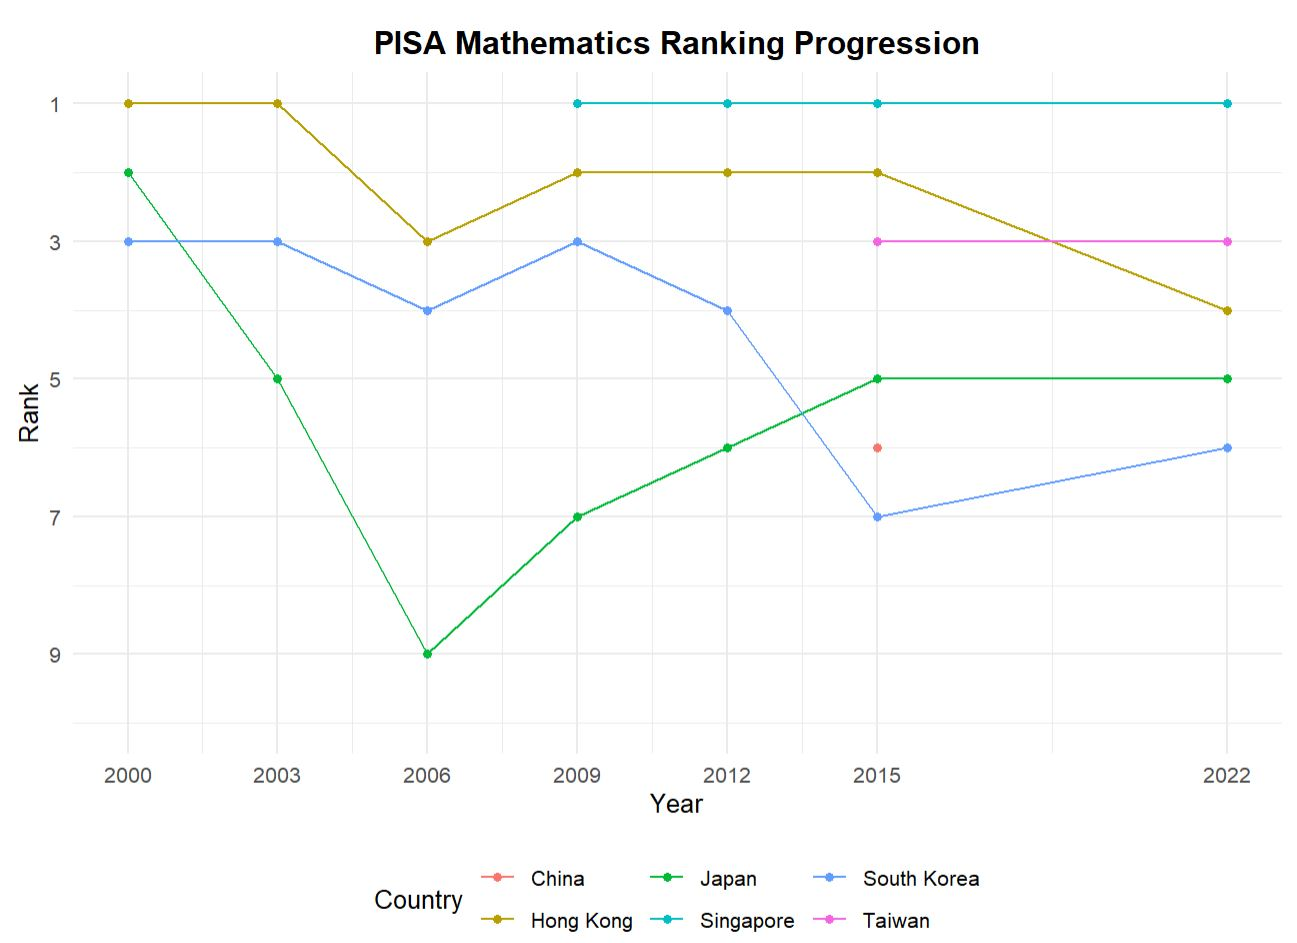
\includegraphics[width=0.8\textwidth]{PISA_maths.JPG}
    \caption{PISA - Maths}
    \label{fig:PISA_Maths}
\end{figure}

\begin{figure}[ht!]
    \centering
        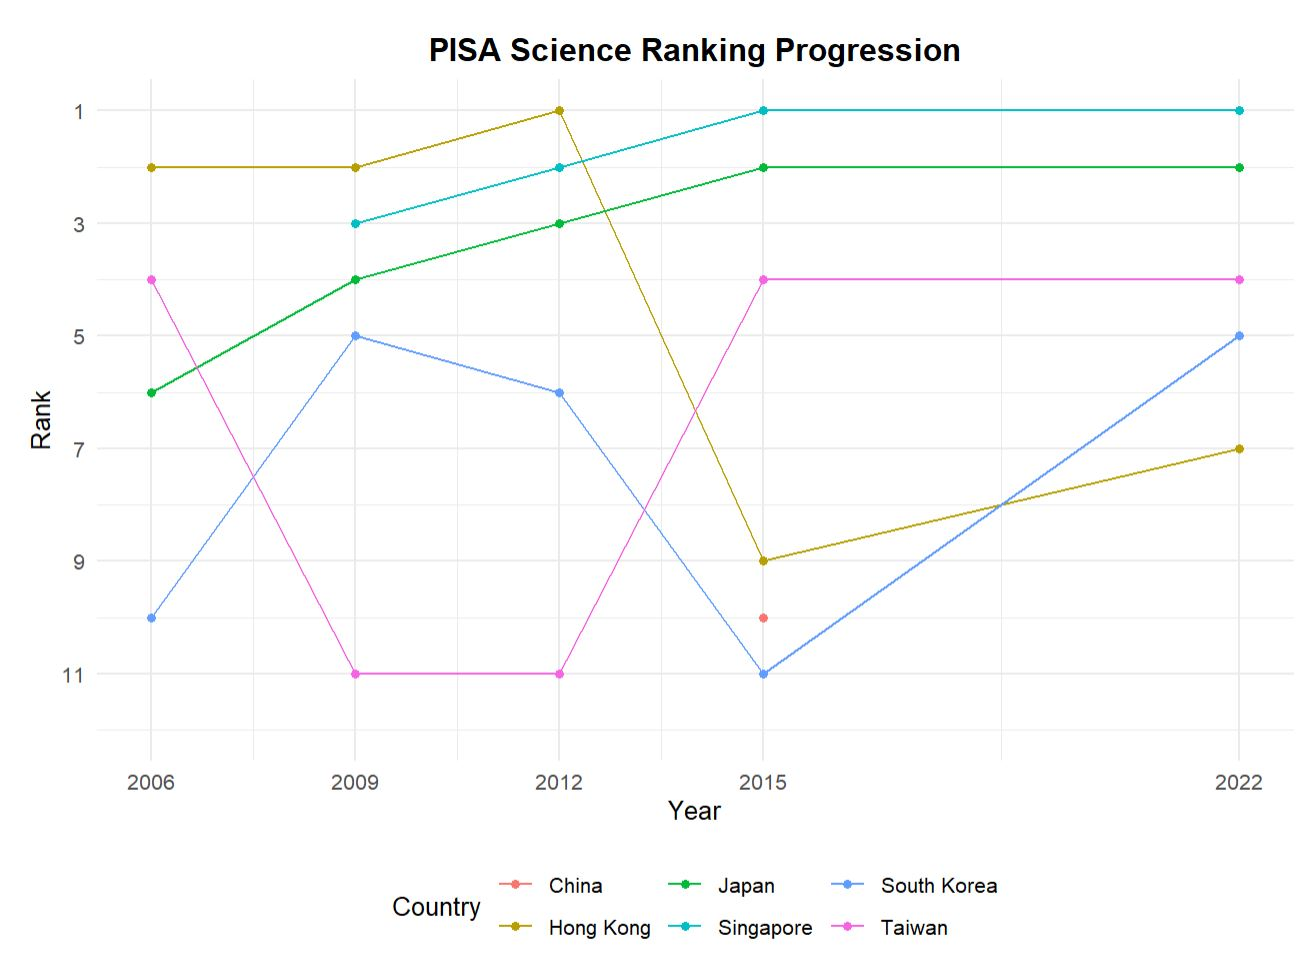
\includegraphics[width=0.8\textwidth]{PISA_science.JPG}
    \caption{PISA - Science}
    \label{fig:PISA_Maths}
\end{figure}

\begin{figure}[ht!]
    \centering
        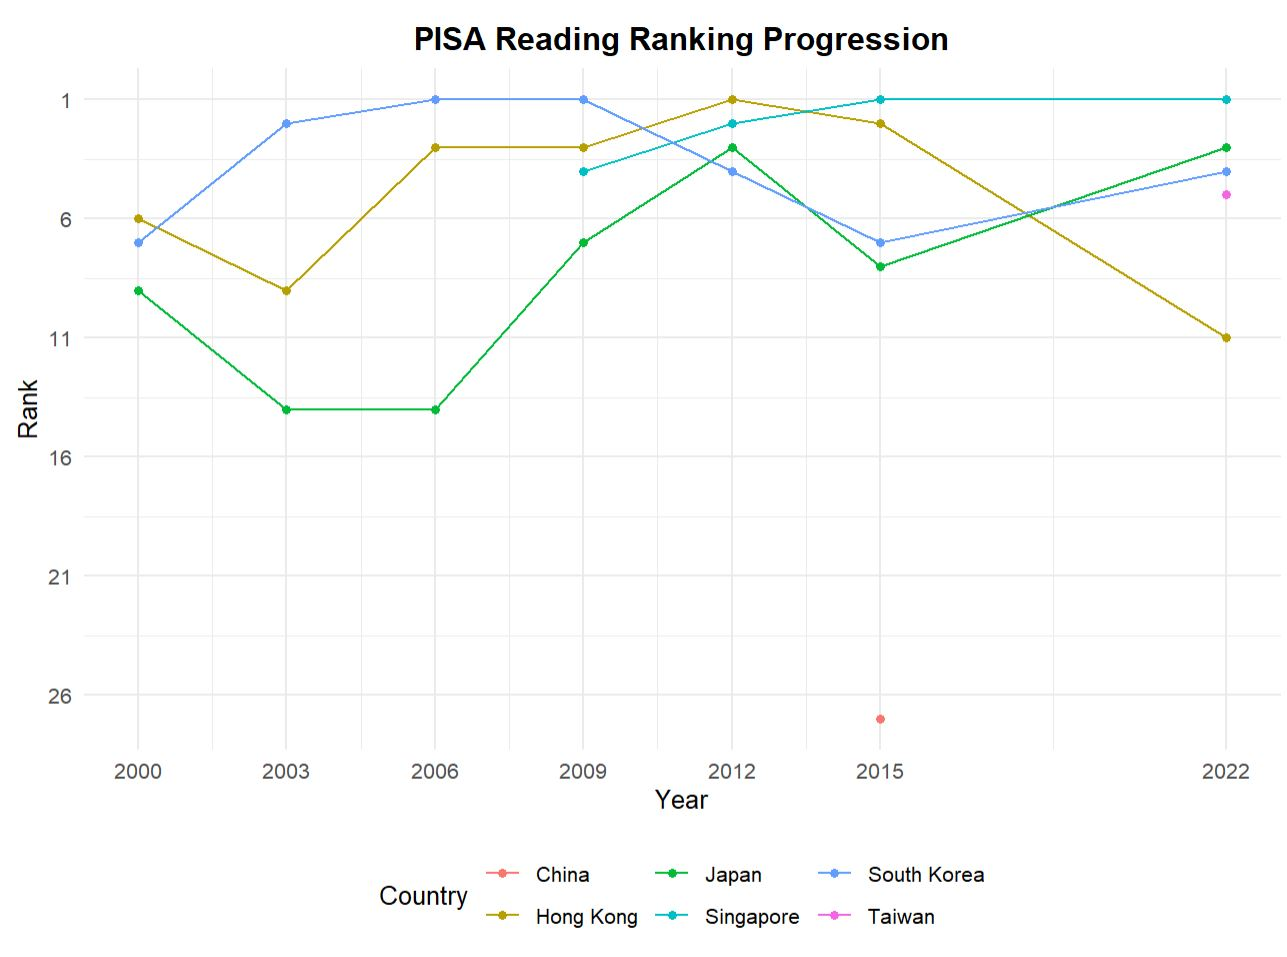
\includegraphics[width=0.8\textwidth]{PISA_reading.JPG}
    \caption{PISA - Reading}
    \label{fig:PISA_Maths}
\end{figure}

\begin{figure}[ht!]
    \centering
        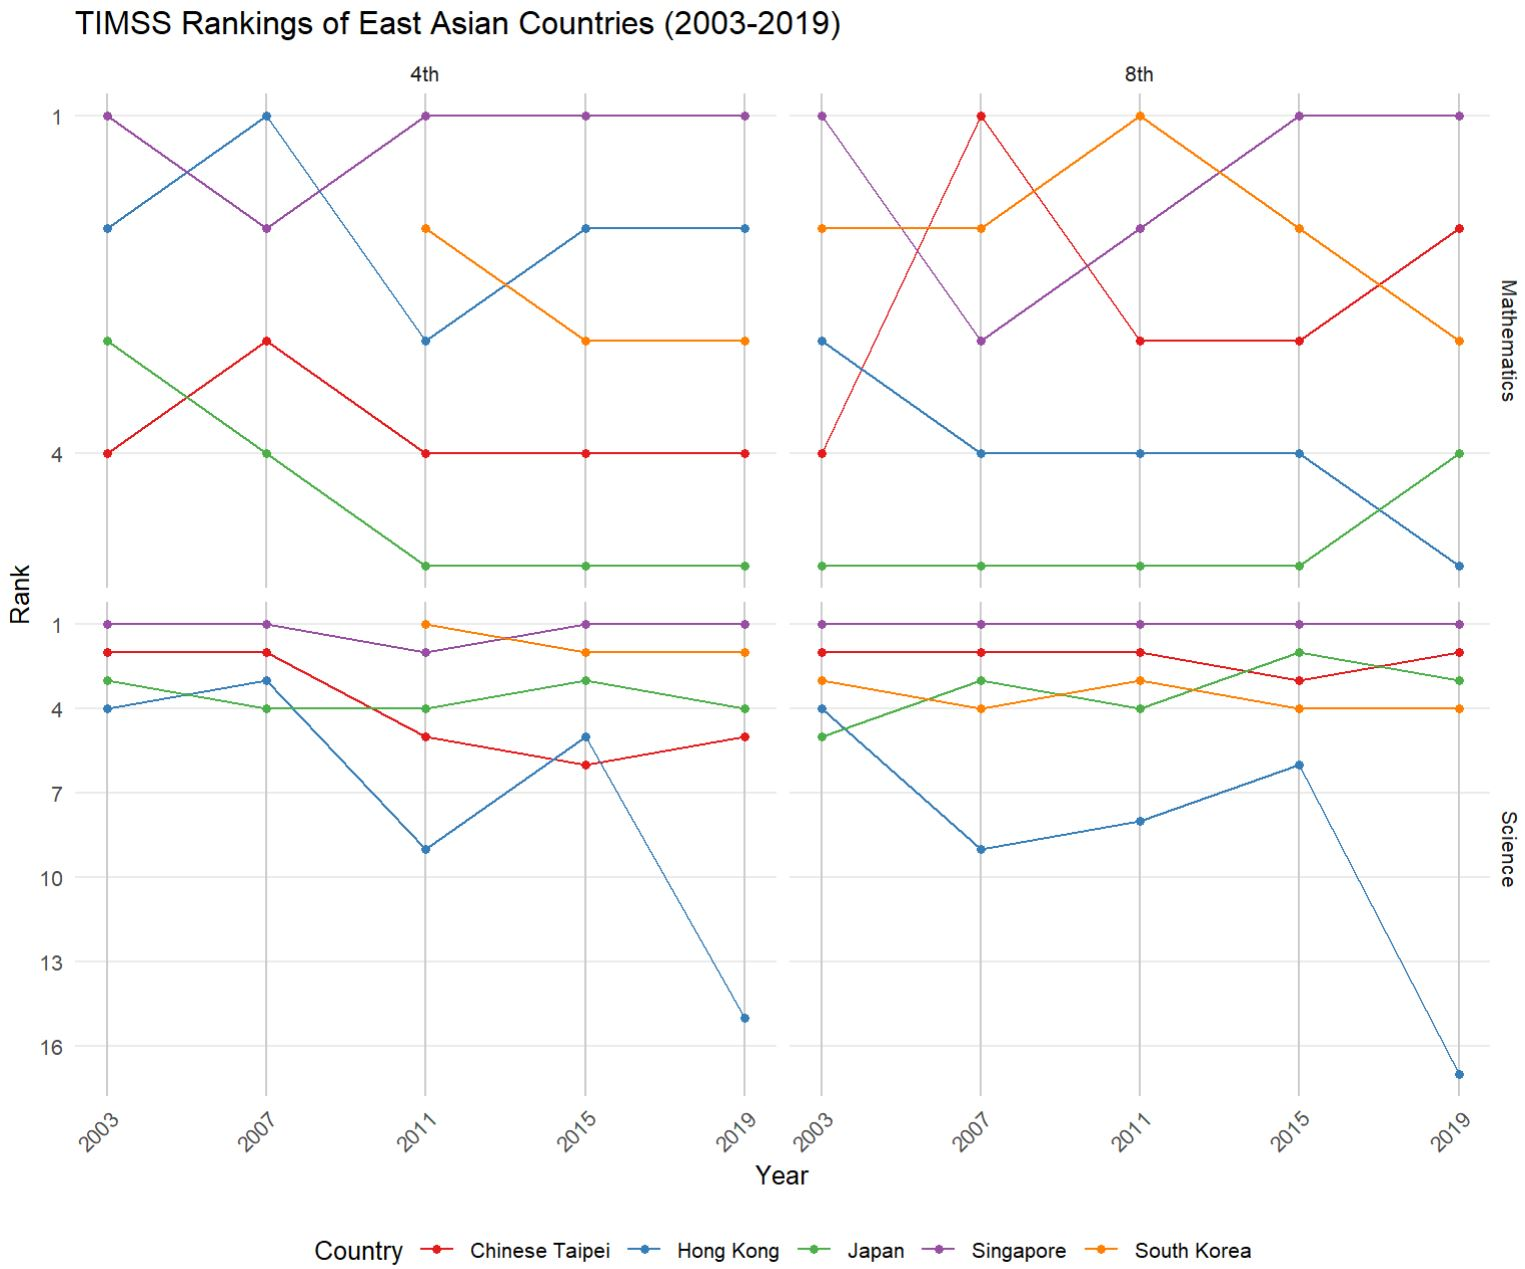
\includegraphics[width=0.8\textwidth]{TIMMS_rank.JPG}
    \caption{TIMSS - Rank}
    \label{fig:TIMMS_RANK}
\end{figure}


\subsubsection{Statistics}
\begin{enumerate}
    \item \hyperlink{https://www.adb.org/sites/default/files/publication/29777/shadow-education.pdf}{China}: The 2004 Urban Household Education and Employment survey covered 4,773 households. It indicated that tutoring was received by 73.8$\%$ of primary, 65.6$\%$ of lower secondary and 53.5$\%$ of upper secondary students. Double Reduction Policy impact (2021): the number of offline after-school tutoring institutions decreased by 84$\%$ from 124,000 to 9,728 within a year of policy implementation; the number of online after-school tutoring institutions decreased by 84$\%$ from 263 to 34 (Ministry of Education of the People's Republic of China, 2022). For-profit Tutoring ban impact: the market value of listed Chinese education companies dropped by \$160 billion within a year of the policy announcement, and student enrollment in K-12 after-school tutoring decreased by approximately 40$\%$ in the first half of 2022 compared to the same period in 2021 (Goldman Sachs Research, 2022).
    \item \hyperlink{https://www.adb.org/sites/default/files/publication/29777/shadow-education.pdf}{Hong Kong}: Government statistics suggest that 34$\%$ of primary and secondary pupils received tutoring in 2006. A 2004–2005 survey of 13,600 households suggested that pupils receiving tutoring were 36.0$\%$ at the primary level, 28.0$\%$ in lower secondary, 33.6$\%$ in middle secondary, and 48.1$\%$ in upper secondary. New senior secondary curriculum impact: the percentage of students receiving private tutoring increased from 34$\%$ in 2006 to 54$\%$ in 2012 (Bray et al., 2014). E-learning implementation (2015): by 2018, 95$\%$ of primary and secondary schools had implemented e-learning in their regular curricula (Education Bureau, Hong Kong, 2019). Extradition Bill protests impact (2019): school suspensions due to protests resulted in a 15-20$\%$ increase in demand for private tutoring services in the latter half of 2019 (South China Morning Post, 2020).
    \item \hyperlink{https://www.adb.org/sites/default/files/publication/29777/shadow-education.pdf}{Japan}: A 2007 survey found that tutorial schools known as juku served 15.9$\%$ of Primary 1 children, that this proportion rose steadily in later grades, and that it reached 65.2$\%$ in Junior Secondary 3. In addition, 6.8$\%$ of Junior Secondary 3 pupils received tutoring at home, and 15.0$\%$ followed correspondence courses. Yutori education impact: the percentage of students attending juku increased from 41.5$\%$ in 2007 to 53.9$\%$ in 2015 for elementary school students, and from 65.2$\%$ to 67.9$\%$ for junior high school students (Ministry of Education, Culture, Sports, Science and Technology - Japan, 2017). COVID-19 impact (2020): the market size of the private tutoring industry decreased by 6.7$\%$ in 2020 compared to 2019, while online learning services saw a 20$\%$ increase in demand during the pandemic (Yano Research Institute, 2021).
    \item \hyperlink{https://kostat.go.kr/board.es?mid=a20111020000&bid=11758&act=view&list_no=424684}{South Korea}: The total private education expenditures of elementary, middle and high school students recorded 26 trillion won in 2022, which rose by 10.8$\%$ from 2021. The private education participation rate stood at 78.3$\%$ in 2022, up 2.8$\%$p from 2021. The weekly participation hours marked 7.2 hours per student in 2022, which grew by 0.5 hours from 2021. The average monthly private education expenditures per student recorded 410 thousand won in 2022, rising by 11.8$\%$ from 2021. The average monthly private education expenditures per participation student recorded 524 thousand won in 2022, rising by 7.9$\%$ from 2021.
    Hagwon Curfew impact: after the implementation of the 10 p.m. curfew in Seoul (2009) and nationwide (2011), the percentage of students receiving private tutoring decreased from 75.0$\%$ in 2009 to 69.4$\%$ in 2012, and the average monthly spending on private tutoring per student decreased from 242,000 won in 2009 to 236,000 won in 2012 (Statistics Korea, 2013). COVID-19 impact (2020): the private education participation rate decreased from 74.8$\%$ in 2019 to 67.1$\%$ in 2020; total private education expenditure decreased by 11.8$\%$ from 2019 to 2020; and online private education participation increased from 14.8$\%$ in 2019 to 39.9$\%$ in 2020. (Statistics Korea, 2021).
    \item Singapore: compulsory education extension (2012): the primary school enrollment rate increased from 99.3$\%$ in 2011 to 99.5$\%$ in 2013 (Ministry of Education, Singapore, 2014). SkillsFuture credit impact: as of 2020, about 500,000 Singaporeans had used their SkillsFuture Credit, with total utilization reaching S\$1 billion (SkillsFuture Singapore, 2021). COVID-19 impact (2020): the private tutoring industry saw a 20-30$\%$ drop in revenue during the circuit breaker period, and online tutoring platforms reported a 100-200$\%$ increase in new sign-ups during the same period (Straits Times, 2020).
\end{enumerate}

Studying the changes in shadow education systems across East Asia from 2009 to 2023 is interesting and important for several reasons. The diverse policy approaches adopted by different countries (e.g., South Korea's hagwon curfew, China's ban on for-profit tutoring) provide a natural experiment to assess the effectiveness of various regulatory strategies. The rapid growth of online tutoring platforms, accelerated by the COVID-19 pandemic, represents a significant shift in the shadow education landscape that calls for investigation. As shadow education can exacerbate educational inequalities, understanding how policy changes have affected access and outcomes across different socioeconomic groups is necessary for informing future policy decisions. The shadow education industry represents a significant economic sector in many East Asian countries. Policy changes can have substantial economic impacts beyond the education sector. As other countries increasingly look to East Asian education systems as models, understanding the role and evolution of shadow education in these high-performing systems has global policy implications.

(Some problems: consistent data across countries and years might be challenging, especially for more recent years. Policies might be implemented in response to existing trends in shadow education, which could bias the results. PISA and TIMSS might not fully capture the extent and nature of shadow education participation. Educational systems and cultural contexts vary significantly across these countries, which might affect the comparability of results. There might be other concurrent policy changes or economic factors affecting educational outcomes. Trends are usually endogenous, and policies might be enacted due to other reasons - not really an anticipation effect but a natural, organic response to internal calls for change)


\subsection{Empirical strategy}

\begin{figure}[htbp]
    \centering
    \begin{sideways}
        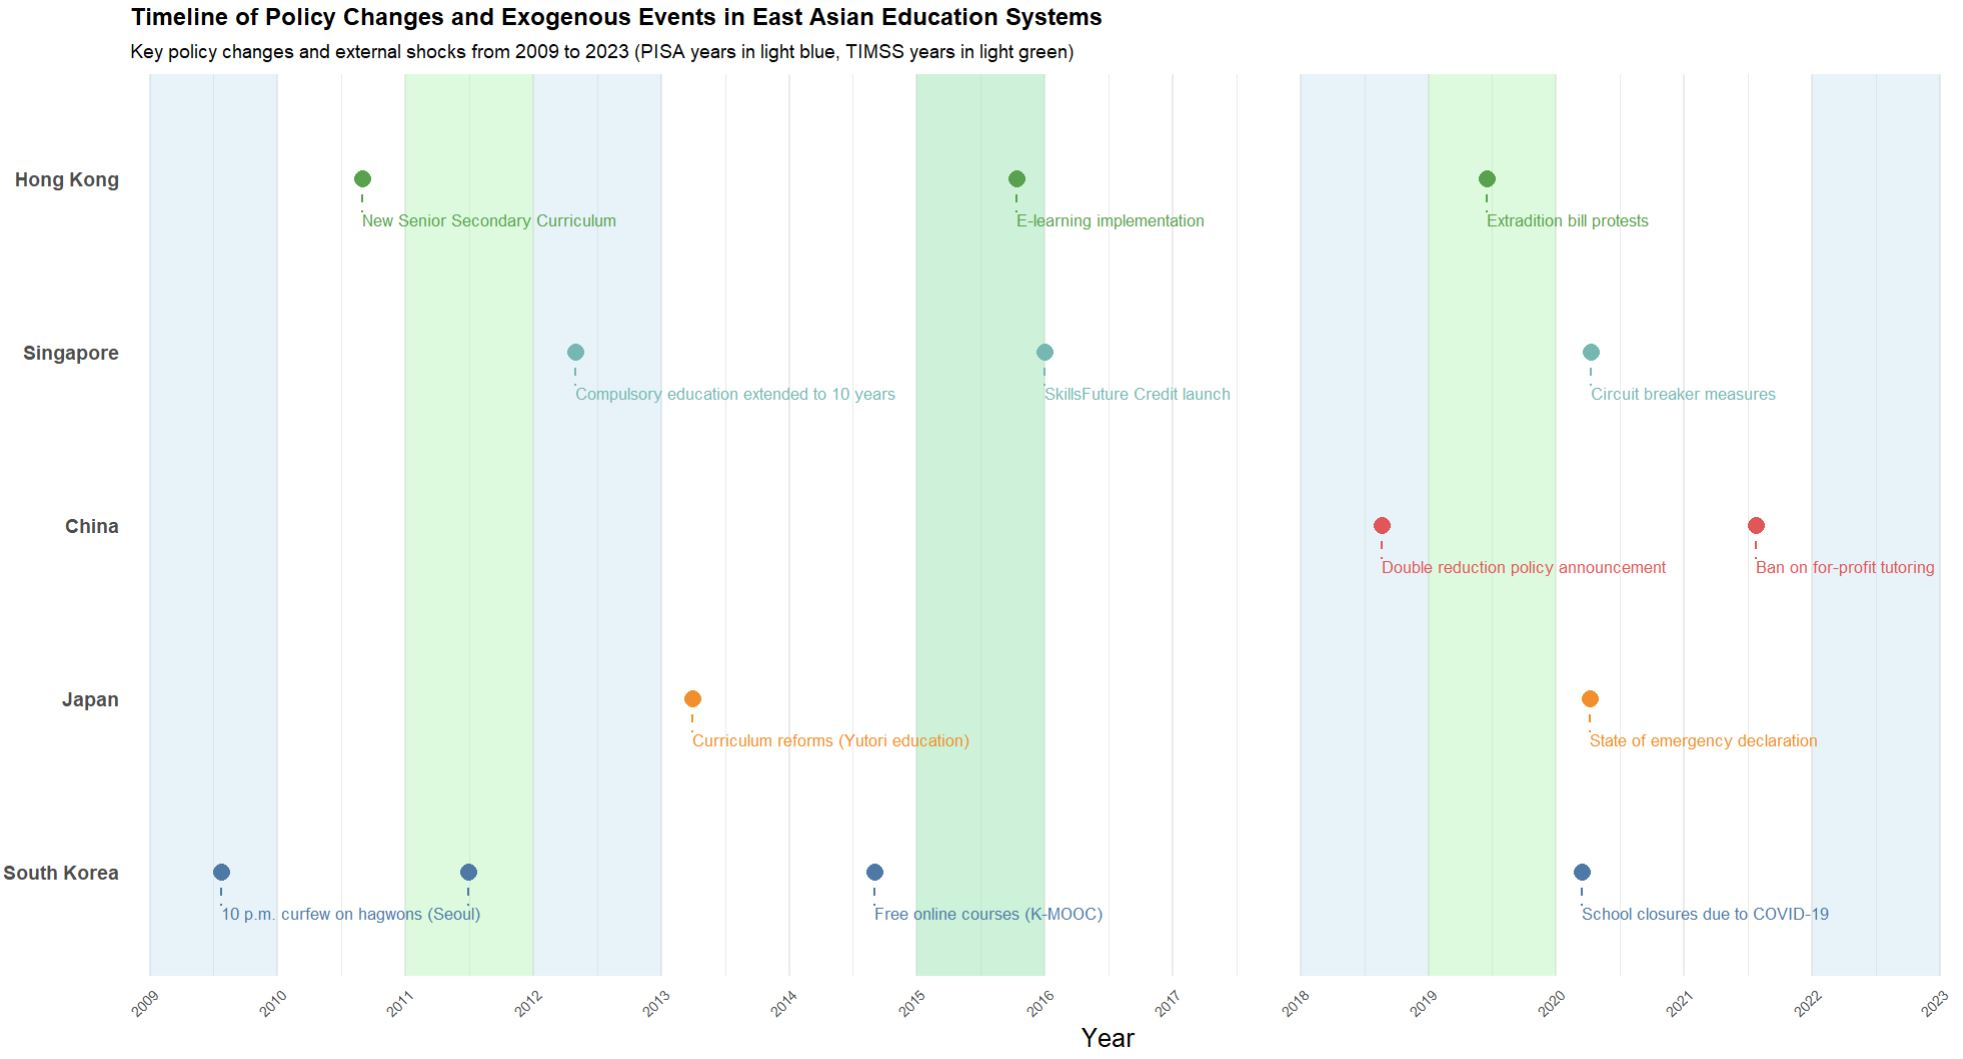
\includegraphics[width=1\textheight]{Capture.JPG}
    \end{sideways}
    \caption{Timeline of changes in shadow education systems in East Asia (2009-2022)}
    \label{fig:timeline}
\end{figure}

\begin{table}[htbp]
\centering
\caption{Timeline of Policy Changes in Shadow Education Systems in East Asia (2009-2023)}
\label{tab:timeline}
\begin{tabular}{llp{7cm}l}
\hline
\textbf{Country} & \textbf{Date} & \textbf{Event} & \textbf{Assessment} \\
\hline
\multirow{5}{*}{South Korea} 
            & July 2009 & 10 p.m. curfew on hagwons (Seoul) & PISA \\
            & June 2011 & Nationwide hagwon curfew & TIMSS \\
            & 2012 & & PISA \\
            & Sept 2014 & Launch of K-MOOC (free online courses) & \\
            & 2015 & & PISA, TIMSS \\
            & 2018 & & PISA \\
            & March 2020 & School closures due to COVID-19 & \\
            & 2022 & & PISA \\
\hline
\multirow{4}{*}{Japan}
            & 2011 & & TIMSS \\
            & 2012 & & PISA \\
            & April 2013 & Curriculum reforms (Yutori education) & \\
            & 2015 & & PISA, TIMSS \\
            & 2018 & & PISA \\
            & 2019 & & TIMSS \\
            & April 2020 & State of emergency declaration (COVID-19) & \\
            & 2022 & & PISA \\
\hline
\multirow{3}{*}{China}
            & Aug 2018 & Double reduction policy announcement & PISA \\
            & July 2021 & Ban on for-profit core subject tutoring & \\
            & 2022 & & PISA \\
\hline
\multirow{6}{*}{Singapore}
            & 2011 & & TIMSS \\
            & May 2012 & Compulsory education extended to 10 years & PISA \\
            & 2015 & & PISA, TIMSS \\
            & Jan 2016 & SkillsFuture Credit launch & \\
            & 2018 & & PISA \\
            & 2019 & & TIMSS \\
            & April 2020 & Circuit breaker measures (COVID-19) & \\
            & 2022 & & PISA \\
\hline
\multirow{6}{*}{Hong Kong}
            & 2009 & & PISA \\
            & Sept 2010 & New Senior Secondary Curriculum & \\
            & 2011 & & TIMSS \\
            & 2012 & & PISA \\
            & Oct 2015 & E-learning implementation & PISA, TIMSS \\
            & 2018 & & PISA \\
            & June 2019 & Extradition bill protests & TIMSS \\
            & 2022 & & PISA \\
\hline
\end{tabular}
\end{table}

\begin{enumerate}
    \item South Korea: 10 p.m. curfew on hagwons (Seoul) - July 25, 2009: Seoul implemented a 10 p.m. curfew on hagwons (private tutoring academies) to reduce study time and stress for students \parencite{lee2011impact}. Nationwide hagwon curfew - June 30, 2011: the curfew policy was extended nationwide, with varying curfew times by region \parencite{bray2014regulating}. Free online courses (K-MOOC) - September 1, 2014: launch of Korea Massive Open Online Courses (K-MOOC) to provide free, high-quality online education \parencite{kim2015efa}. School closures due to COVID-19 - March 15, 2020: nationwide school closures and shift to online learning in response to the pandemic \parencite{kim2020school}.
 
 \item Japan: curriculum reforms (Yutori education) - April 1, 2013: implementation of new curriculum guidelines emphasizing "relaxed education" or "Yutori kyōiku" \parencite{bjork2019high}. State of emergency declaration - April 7, 2020: first COVID-19 state of emergency declared, affecting education nationwide \parencite{yamamoto2010cultural}.

\item China: Double reduction policy announcement - August 22, 2018: China announced plans to reduce students' academic burden and after-school tutoring hours \parencite{chen2024examining}. Ban on for-profit tutoring - July 24, 2021: China banned for-profit tutoring in core school subjects to ease pressure on children and parents \parencite{chinalawtranslate2021}.

\item Singapore: compulsory education extended to 10 years - May 1, 2012: Singapore extended compulsory education from 6 to 10 years \parencite{ministry2012compulsory}. SkillsFuture credit launch - January 1, 2016: the SkillsFuture Credit initiative in Singapore, launched in 2016, is a government program designed to encourage Singaporeans to engage in lifelong learning by providing them with credits to use for approved skills training courses \parencite{skillsfuture2016credit}. Circuit breaker measures - April 8, 2020: implementation of strict lockdown measures, including closure of schools and shift to full home-based learning \parencite{ministry2020homebased}.

\item Hong Kong: New senior secondary curriculum - September 1, 2010: in 2009, the Education Bureau of the Hong Kong Special Administrative Region (HKSAR) introduced the New Academic Structure (NAS) for Senior Secondary Education and Higher Education. This reform aimed to align Hong Kong's education system with international standards and improve the overall quality of education \parencite{educationbureau2009nas}. E-learning implementation - October 13, 2015: launch of the Fourth Strategy on Information Technology in Education to promote e-learning in schools \parencite{educationbureau2009nas}. Extradition bill protests - June 18, 2019: large-scale protests began, affecting the education system and leading to school suspensions \parencite{pang2020gazing}.
\end{enumerate}

\subsection{Identification strategy}

Idea: to leverage the staggered implementation of shadow education policies across East Asian countries between 2009 and 2023 by employ a DiD approach (variation in the timing and nature of policy changes across countries $->$ identify causal effects).

\begin{equation}
    Y_{ict} = \beta_0 + \beta_1(\text{Policy}_{ct}) + \beta_2(\text{Post}_t) + \beta_3(\text{Policy}_{ct} \times \text{Post}_t) + \gamma_c + \delta_t + \varepsilon_{ict}
\end{equation}

$Y_{ict}$ is the outcome for individual $i$ in country $c$ at time $t$, $\text{Policy}_{ct}$ is a dummy for whether the policy is in effect in country $c$ at time $t$, $\text{Post}_t$ is a dummy for the post-treatment period, and $\gamma_c$ and $\delta_t$ are country and time fixed effects.

By employing this strategy we can use countries without policy changes as control groups while exploiting multiple "experiments" due to staggered policy implementation. We can also control for time-invariant country characteristics and common time trends.

\subsection{Model}

1. Students:

Objective function:
\begin{equation}
    \max_{E,T} U_s = \alpha A - \beta E
\end{equation}

Constraints:
\[
\begin{aligned}
A &= f(E, T, S) \\
E &\geq 0 \\
T &\geq 0
\end{aligned}
\]

Where:
$A$ is academic achievement, $E$ is student effort, $T$ is hours of tutoring, $S$ is school quality, $\alpha$ and $\beta$ are weights for achievement and effort.

2. Parents:

Objective function:
\begin{equation}
    \max_{T} U_p = \gamma A - \delta C
\end{equation}

Constraints:
\[
\begin{aligned}
    C &= pT \\
    pT &\leq I \\ 
T &\geq 0
\end{aligned}
\]

Where: $C$ is the cost of tutoring, $p$ is the price per hour of tutoring, $I$ is the income allocated for education, $\gamma$ and $\delta$ are weights for achievement and costs

3. Tutors:

Objective function:
\begin{equation}
    \max_{E_t,T} U_t = \varepsilon I - \zeta E_t
\end{equation}

Constraints:
\[
\begin{aligned}
I &= pT \\
E_t &\geq 0 \\
T &\geq 0
\end{aligned}
\]

Where: $I$ is income from tutoring, $E_t$ is tutor effort, $\varepsilon$ and $\zeta$ are weights for income and effort

4. Schools:

Objective function:
\begin{equation}
    \max_{S} U_{sch} = \eta \sum_{i=1}^n A_i
\end{equation}


Constraints:
\[
\begin{aligned}
S &\leq S_{max} \\
S &\geq 0
\end{aligned}
\]

Where: $\sum_{i=1}^{n} A_i$ is aggregated students' academic achievement, $S_{max}$ represents the maximum school quality achievable given resources, $\eta$ is the weight for overall performance

To solve this system, we need to specify the functional form of $A = f(E, T, S)$. If we assume a Cobb-Douglas form:

\[
A = kE^{\alpha_1}T^{\alpha_2}S^{\alpha_3}
\]

Where $k$ is a constant and $\alpha_1 + \alpha_2 + \alpha_3 = 1$ for constant returns to scale.

Now, we can derive the first-order conditions for each agent:

1. Students:
\[
\frac{\partial U_s}{\partial E} = \alpha k\alpha_1 E^{\alpha_1-1}T^{\alpha_2}S^{\alpha_3} - \beta = 0
\]
\[
\frac{\partial U_s}{\partial T} = \alpha k\alpha_2 E^{\alpha_1}T^{\alpha_2-1}S^{\alpha_3} = 0
\]

2. Parents:
\[
\frac{\partial U_p}{\partial T} = \gamma k\alpha_2 E^{\alpha_1}T^{\alpha_2-1}S^{\alpha_3} - \delta p = 0
\]

\begin{equation}
    A = kE^{\alpha_1} T^{\alpha_2} S^{\alpha_3}
\end{equation}

\begin{equation}
    \frac{\partial U_s}{\partial E} = \alpha k \alpha_1 E^{\alpha_1-1} T^{\alpha_2} S^{\alpha_3} - \beta = 0
\end{equation}

\begin{equation}
    \frac{\partial U_p}{\partial T} = \gamma k \alpha_2 E^{\alpha_1} T^{\alpha_2-1} S^{\alpha_3} - \delta p = 0
\end{equation}

3. Tutors:
\[
\frac{\partial U_t}{\partial E_t} = -\zeta = 0
\]
\[
\frac{\partial U_t}{\partial T} = \varepsilon p = 0
\]

4. Schools:
\[
\frac{\partial U_{sch}}{\partial S} = \eta n k\alpha_3 E^{\alpha_1}T^{\alpha_2}S^{\alpha_3-1} = 0
\]

It is a system that can be solved simultaneously to find the equilibrium values of $E$, $T$, $E_t$, and $S$. The solution will depend on the specific parameter values and may require numerical methods to solve. By writing it like that, the formalization allows for many extensions such as: comparative statics to examine how changes in parameters affect equilibrium outcomes; the incorporation of policy constraints (e.g., maximum tutoring hours); the introduction of uncertainty or asymmetric information; and the analysis of different market structures in the tutoring industry.

Considering schools as cost minimizers and profit maximizers would add an important dimension to the model, especially when analyzing the interaction between formal education systems and shadow education. However, it is context-specific.

Public Schools:
For public schools, a pure profit maximization model may not make sense:

a) Cost minimizers subject to a quality constraint:
\[
\min_{I} C = f(I) \quad \text{subject to} \quad S \geq S_{min}
\]

Where C is cost, I is inputs (teachers, resources), and $S_{min}$ is a minimum quality standard.

b) Quality maximizers subject to a budget constraint:
\[
\max_{I} S = g(I) \quad \text{subject to} \quad C \leq B
\]
Where B is the school's budget.

Private schools:
For private schools, a profit maximization model could make sense:
\[
\max_{P,S} \pi = PR - C(S)
\]
Where $\pi$ is profit, P is tuition price, R is enrollment, and C(S) is the cost function depending on school quality S.

Hybrid model: an ojective function that balances profit/cost considerations with educational outcomes:
\[
\max_{S} U_{sch} = \omega \pi + (1-\omega) \eta \sum_{i=1}^{n} A_i
\]
Where $\omega$ is a weight between 0 and 1, representing the balance between financial and educational objectives.

\subsection{External validity}

Including South Korea, Japan, China, Singapore, and Hong Kong provides variation in cultural and educational contexts. Covering 2009-2023 allows for analysis of both short-term and long-term effects. From curfews to online tutoring growth, we can capture various aspects of shadow education systems.
This diversity increases the generalizability of our findings beyond a single country or policy context. 

\subsection{Identification threats:}

a) Policy endogeneity: policies might be implemented in response to existing trends. Maybe we can use pre-policy trends analysis and placebo tests to address this endogeneity issues.

b) Spillover effects: policies in one country might affect behavior in neighboring countries. Maybe we can use spatial econometric techniques to model these spillovers.

c) IV: maybe we can use political changes or historical events as instruments for policy implementation, e.g., changes in government might lead to education policy changes for reasons unrelated to shadow education trends.

d) RDD: for policies with clear age or date cutoffs (e.g., the hagwon curfew in South Korea), maybe we can use a RDD, which would involve comparing outcomes for students just above and below the cutoff.

\section{A few other ideas}

1) A dynamic shadow education model:

$\max_{E_t, T_t} \sum_{t=0}^{T} \beta^t [U_s(A_t, E_t)]$ \\

\text{subject to:}
$A_t = f(E_t, T_t, S_t, A_{t-1})
E_t, T_t \geq 0$

\text{where:} \\
$\beta$ \text{ is the discount factor}\\
$A_t$ \text{ is academic achievement in period t}\\
$E_t$ \text{ is student effort in period t}\\
$T_t$ \text{ is tutoring hours in period t}\\
$S_t$ \text{ is school quality in period t}\\

2) Risk-averse U(f):

\text{Students: } $U_s = E[u(A)] - v(E)$ \text{, where u is concave} \\

\text{Parents: } $U_p = E[w(A)] - x(C)$ \text{, where w is concave} \\

\text{where:} $E[\cdot]$ \text{ denotes expected value} \\
$u$ \text{ and w are concave utility functions} \\
$v$ \text{ and x are convex cost functions} \\

3) Labor market extension: 

$W = g(A, \theta)$ \\
\text{where:} \\
$W$ \text{ is wage} \\
$g$ \text{ is a function mapping academic achievement to wages} \\
$\theta$ \text{ represents labor market conditions} \\

4) General equilibrium effects: a simple general equilibrium model that includes: a production sector using skilled labor (affected by education), an education sector (including shadow education), and households making education decisions.


\printbibliography

\end{document}
